% !TeX encoding = UTF-8
% !TeX spellcheck = pl_PL
\documentclass[polish, titlepage, 12pt]{article}

\usepackage[svgnames]{xcolor}
\usepackage[nosingleletter, lastparline]{impnattypo}
\usepackage[polish]{babel}
\usepackage{csquotes}
\usepackage[backref, backend=bibtex]{biblatex}
\usepackage[breaklinks]{hyperref}
\usepackage{bookmark}
\usepackage[babel, tracking]{microtype}
\usepackage{booktabs}
\usepackage[margin=1in]{geometry}
\usepackage{graphicx}
\usepackage{parskip}
\usepackage{framed}
\usepackage{tabularx}
\usepackage{ltablex}
\usepackage{adjustbox}
\usepackage{float}
\usepackage{longtable}
\usepackage{subcaption}
\usepackage[strings]{underscore}
\usepackage{tikz}
\usepackage{amsmath}
\usepackage{xfrac,unicode-math}
\usepackage{physics}
\usepackage{wrapfig}

\linespread{1.5}

\title{Transformacja Fouriera}
\author{Piotr Rogulski}
\date{\today}

\addbibresource{fourier.bib}

\begin{document}

\maketitle

\tableofcontents

\newpage



\section{Rys historyczny}
\begin{wrapfigure}{r}{0.35\textwidth}
    \centering
    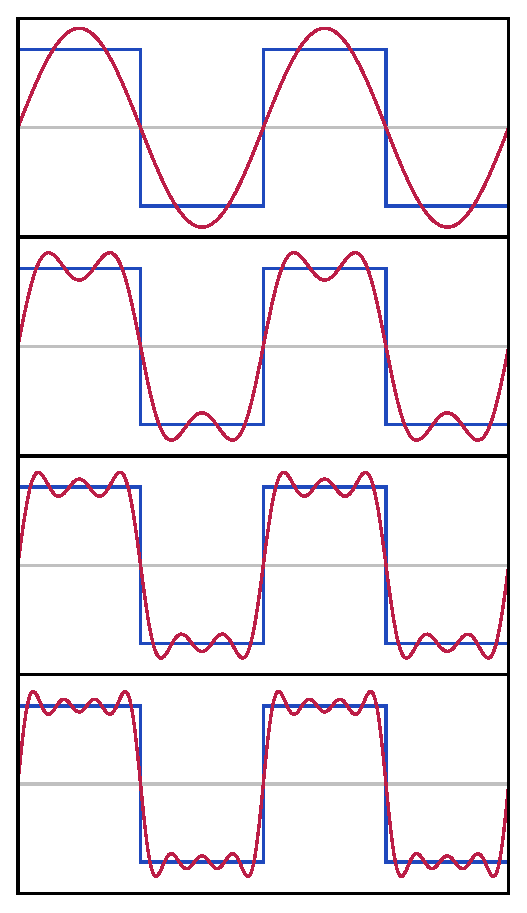
\includegraphics[width=0.33\textwidth]{img/fourier-series.eps}
\end{wrapfigure}
Transformacja Fouriera zawdzięcza swoją nazwę Josephowi Fourierowi, który w 1822 roku
opublikował swoją pracę \textit{Théorie analytique de la chaleur} (pol.\ \textit{Analityczna teoria ciepła}).
W niej twierdził, że dowolną funkcję okresową można przedstawić jako sumę szeregu trygonometrycznego.
O ile ta teza nie jest prawdziwa bez dodatkowych założeń, to stanowiła ona podstawę do wielu
rodzajów transformacji Fouriera. Wcześniej, w 1807 roku, Fourier opublikował swoją pracę
\textit{Mémoire sur la propagation de la chaleur dans les corps solides}
(pol.\ \textit{Rozprawa o propagacji ciepła w ciałach stałych}), która to wprowadziła
analizę Fouriera oraz szereg Fouriera. Fourier wprowadził ten szereg w celu rozwiązania
równania ciepła, które jest równaniem różniczkowym cząstkowym. Później jednak okazało się,
że te same metody mogą być stosowane do rozwiązywania przeróżnych problemów fizycznych i
matematycznych.



\section{Transformacja Fouriera}
Transformacja Fouriera jest operatorem liniowym o typie
\( \mathcal{F}: (\mathbb{R}^n \to \mathbb{R}^n) \to (\mathbb{R}^n \to \mathbb{R}^n) \).
Przekształca ona funkcję operującą w dziedzinie czasu na funkcję operującą w dziedzinie częstotliwości.

\begin{equation}\label{eq:ft-n}
    \mathcal{F}(f)(\symbf{\xi}) = \int_{\mathbb{R}^n} f(\symbf{x}) e^{-2\pi i (\symbf{x \cdot \xi})} d\symbf{x}
\end{equation}

Ogólna postać definicji transformacji Fouriera (\ref{eq:ft-n}) pozwala na zdefiniowanie jej
dla funkcji o argumencie o dowolnym wymiarze. W wielu zastosowaniach korzysta się jednak
z jednowymiarowej transformacji Fouriera:

\begin{equation}\label{eq:ft-1}
    \mathcal{F}(f)(\xi) = \int_{-\infty}^{\infty} f(x) e^{-2\pi i x \xi} dx
\end{equation}


\subsection{Własności transformacji Fouriera}
\begin{itemize}
    \item liniowość: \( \mathcal{F}(af + bg) = a\mathcal{F}f + b\mathcal{F}g \)
    \item przesunięcie: \( \mathcal{F}(f(x - a)) = e^{-2\pi i a \xi} \mathcal{F}f(\xi) \)
    \item modulacja: \( \mathcal{F}(e^{2\pi i a x} f(x)) = \mathcal{F}f(\xi - a) \)
    \item symetria: \( \mathcal{F}(\mathcal{F}f)(x) = f(-x) \)
    \item splot: \( \mathcal{F}(f * g) = \mathcal{F}f \cdot \mathcal{F}g \)
    \item pochodna: \( \mathcal{F}(f') = 2\pi i \xi \mathcal{F}f \)
\end{itemize}



\section{Dyskretna transformacja Fouriera}

Podstawowa transformata Fouriera jest zdefiniowana dla funkcji ciągłych.
Często jednak dostępne wartości nie mają charakteru ciągłego, lecz są próbkowane.
W tym celu zdefiniowany został dyskretny odpowiednik transformacji Fouriera (DFT).

\begin{equation}\label{eq:dft-n}
    X_{\symbf{k}} = \sum_{\symbf{n} = \symbf{0}}^{\symbf{N} - \symbf{1}} x_{\symbf{n}} e^{-2\pi i \frac{\symbf{k \cdot n}}{\symbf{N}}}
\end{equation}

W postaci jednowymiarowej:

\begin{equation}\label{eq:dft-1}
    X_k = \sum_{n=0}^{N-1} x_n e^{-2\pi i \frac{kn}{N}}
\end{equation}

\subsection{Macierz DFT}
Definicja (\ref*{eq:dft-1}) pozwala na zapisanie dyskretnej transformacji Fouriera
w postaci macierzowej:

\begin{equation}\label{eq:dft-matrix-eq}
    X_k = \sum_{n=0}^{N-1} x_n e^{-2\pi i \frac{kn}{N}}
    \Longleftrightarrow X = Wx,
    \qquad \text{gdzie} \quad
    W_{kn} = e^{-2\pi i kn / N}
\end{equation}

Elementy macierzy \(W\) są postaci \( w_{kn} = \omega^{kn} \), gdzie \( \omega = e^{-2\pi i / N} \):

\begin{equation}\label{eq:dft-matrix}
    W = \begin{bmatrix}
        1 & 1 & 1 & \cdots  & 1 \\
        1 & \omega & \omega^2 & \cdots  & \omega^{N-1} \\
        1 & \omega^2 & \omega^4 & \cdots  & \omega^{2(N-1)} \\
        \vdots & \vdots & \vdots & \ddots & \vdots \\
        1 & \omega^{N-1} & \omega^{2(N-1)} & \cdots  & \omega^{(N-1)(N-1)}
    \end{bmatrix}
\end{equation}

Jest to symetryczna macierz Vandermonde'a dla pierwiastka z jedności: \(\omega^N = 1\).
Jeżeli dodatkowo jej elementy zostaną przeskalowane przez \(1/\sqrt{N}\), to otrzymamy macierz
unitarną. Wtedy DFT staje się transformacją unitarną, co pozwala myśleć o niej jako o
obrocie układu współrzędnych.



\section{Szybka transformacja Fouriera}
Obliczanie dyskretnej transformacji Fouriera zgodnie z definicją (\ref{eq:dft-1}) wymaga
\( \mathcal{O}(N^2) \) operacji. Istnieją jednak algorytmy, które pozwalają na obliczenie
DFT w lepszym czasie. Jednym z nich jest algorytm Cooleya-Tukeya z 1965 roku, który wymaga
\( \mathcal{O}(N \log N) \) operacji.

Jest to algorytm typu \textit{dziel i zwyciężaj}. Pozwala on obliczyć DFT dla
\(N = N_1 N_2\) elementów za pomocą dwóch DFT dla \(N_1\) i \(N_2\) elementów.
Z tego powodu najlepiej sprawuje się dla liczb ,,gładkich'', czyli takich, które mają
wiele małych dzielników --- osiąga wtedy złożoność \( \mathcal{O}(N \log N) \)
(patrz rys.\ \ref{fig:fft-diagram-radix2}).

\begin{figure}[htbp]
    \centering
    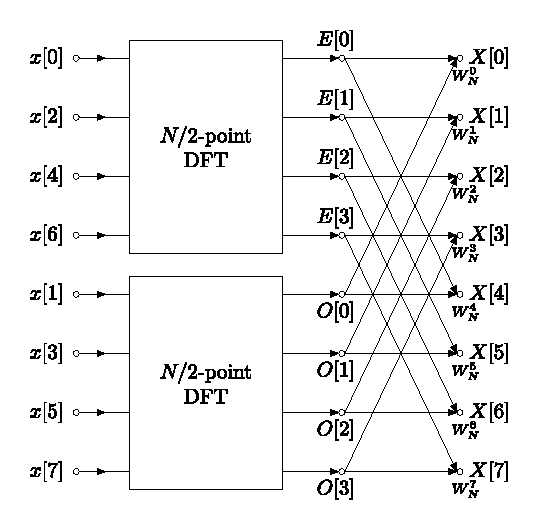
\includegraphics[width=0.5\linewidth]{img/fft-diagram.eps}
    \caption{Schemat FFT dla decymacji Radix-2}\label{fig:fft-diagram-radix2}
\end{figure}

Nie jest to jednak jedyny algorytm obliczania FFT.\@ Innym przykładem jest algorytm Bluesteina,
który wykorzystuje Chirp Z-transform --- polega on na próbkowaniu sygnału wzdłuż krzywych
na płaszczyźnie zespolonej zamiast wzdłuż okręgów, jak w przypadku DFT (rys.\ \ref{fig:chirp-z}).
Istnieje także algorytm Radera, który optymalizuje operacje na macierzy DFT poprzez sprowadzenie
jej do postaci cyklicznej (rys.\ \ref{fig:rader}).

\begin{figure}[htbp]
    \begin{adjustbox}{center}
        \begin{minipage}[t][][b]{0.6\textwidth}
            \centering
            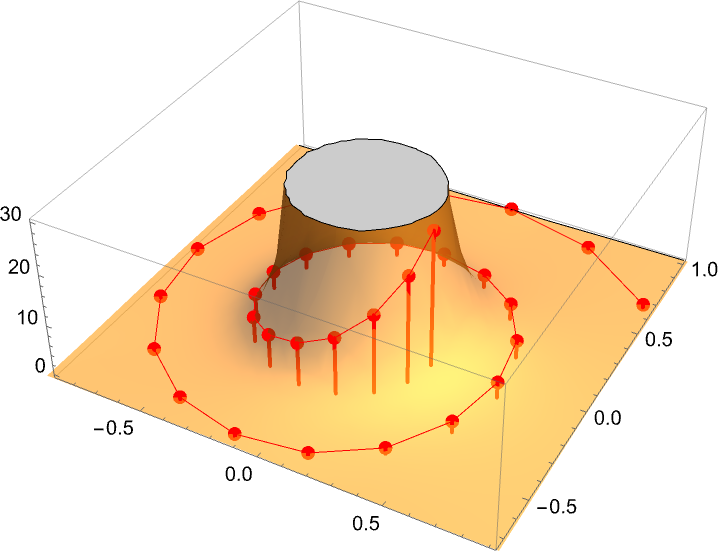
\includegraphics[width=0.8\linewidth]{img/chirp-z.png}
            \captionof{figure}{Chirp Z-transform}\label{fig:chirp-z}
        \end{minipage}%
        \begin{minipage}[t][][b]{0.6\textwidth}
            \centering
            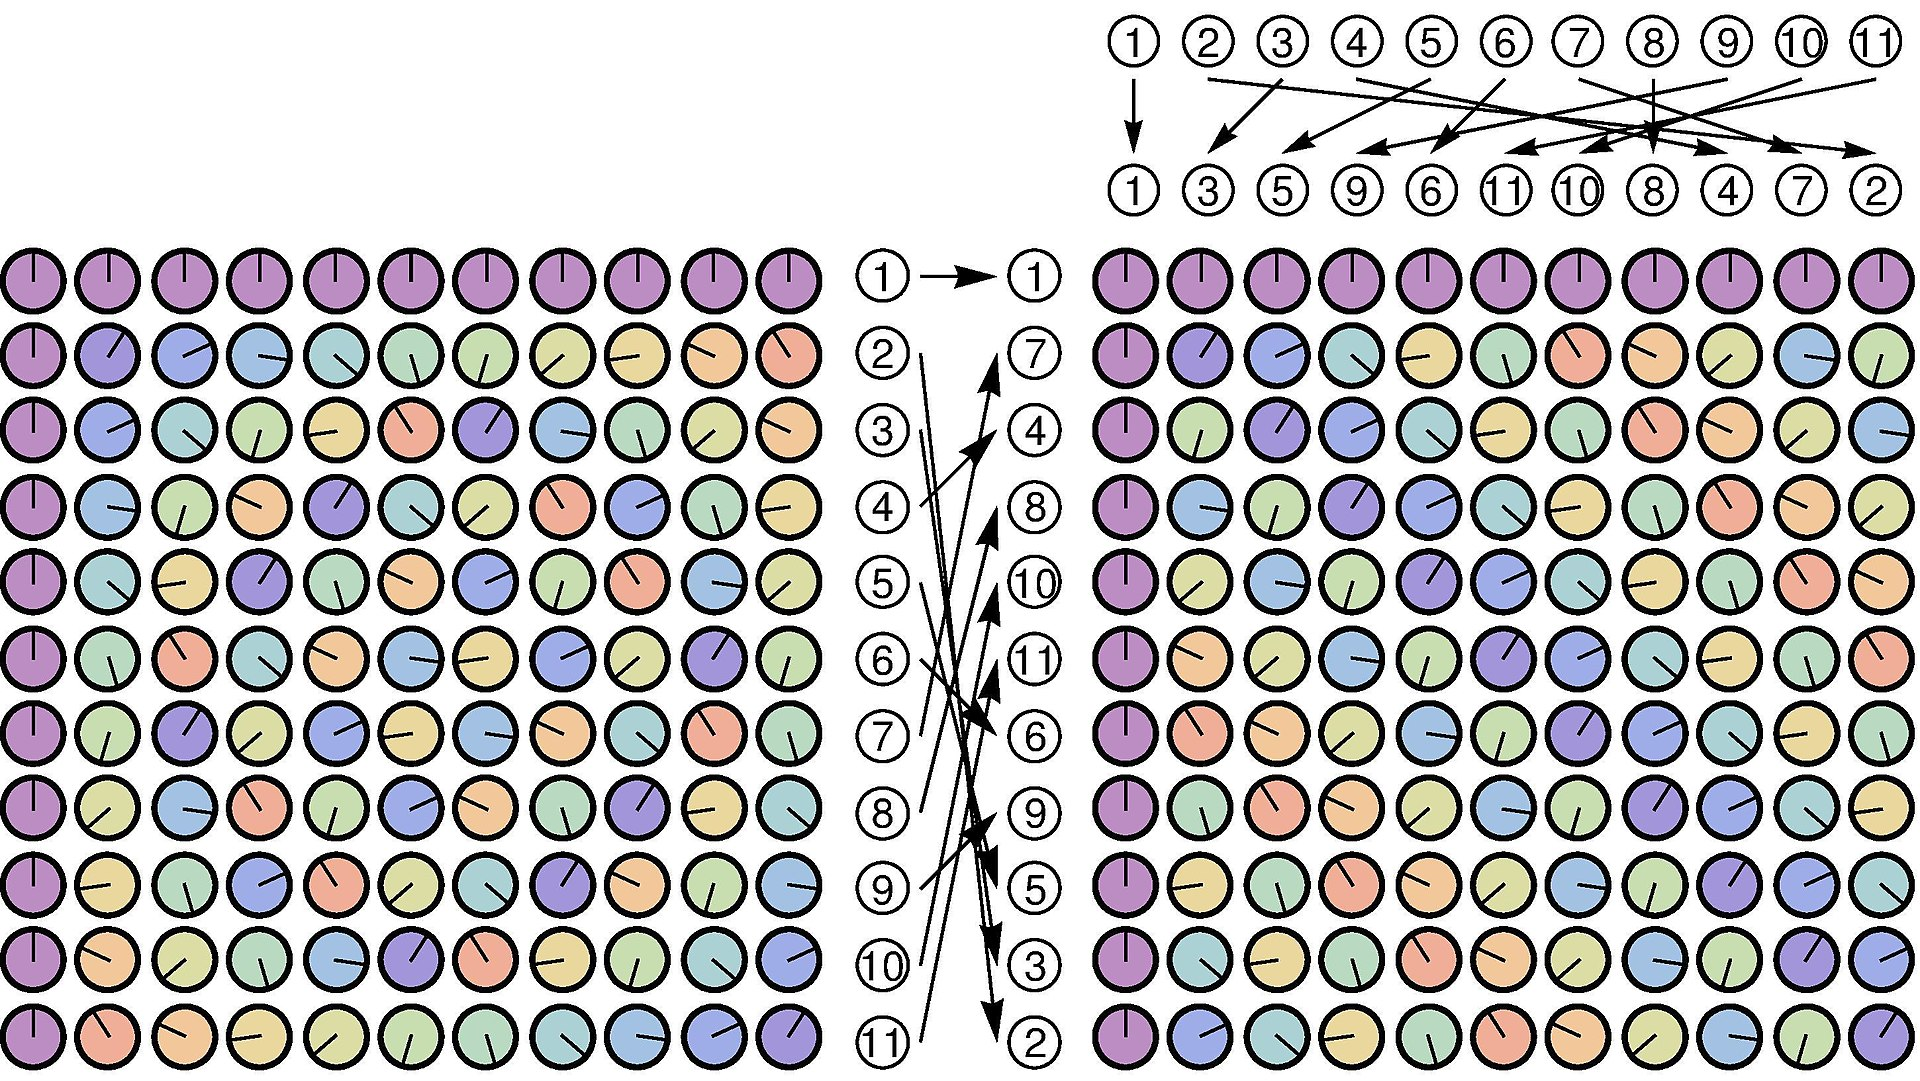
\includegraphics[width=0.8\linewidth]{img/rader.jpg}
            \captionof{figure}{Algorytm Radera}\label{fig:rader}
        \end{minipage}
    \end{adjustbox}
\end{figure}



\section{Zastosowania}

% \subsection{Spektroskopia}

% \subsection{FTIR}

% \subsection{Analiza równań różniczkowych}

% \subsection{Discrete cosine transform}

\newcommand{\usage}[2]{
    \item \textbf{#1} \\
          #2
}

\begin{itemize}
    \setlength\itemsep{1em}
    \usage{Spektroskopia fourierowska}{
        W spektroskopii fourierowskiej do analizy widm wykorzystuje się transformację Fouriera.
        Zamiast bezpośredniej obserwacji widma, korzysta się z interferometru.
        Pozwala on na badanie intensywności sygnału w zależności od częstotliwości (a więc i długości fali).
    }
    \usage{Analiza równań różniczkowych}{
        Transformacja Fouriera pozwala uprościć rozwiązywanie równań różniczkowych.
        Sprowadza ona równania różniczkowe do równań algebraicznych.

        Przykład: oscylator harmoniczy

        \[
            \dv[2]{x}{t} + 2\gamma \dv{x}{t} + \omega_0^2 x(t) = \frac{f(t)}{m}
        \]
        \[
            -\omega^2 X(\omega) - 2i\gamma\omega X(\omega) + \omega_0^2 X(\omega)
            = \frac{F(\omega)}{m},
            \quad \text{gdzie} \quad
            X(\omega) = \mathcal{F}(x(t)), F(\omega) = \mathcal{F}(f(t))
        \]
        \[
            X(\omega) = \frac{F(\omega)}{m(\omega_0^2 - \omega^2 - 2i\gamma\omega)}
        \]
        \[
            x(t) = \frac{1}{2\pi} \int_{-\infty}^{\infty} X(\omega) e^{i\omega t} d\omega
        \]
    }
    \usage{Discrete cosine transform}{
        Dyskretna transformacja kosinusowa jest podobna do dyskretnej transformacji Fouriera.
        Różni się ona tym, że operuje na liczbach rzeczywistych, a nie zespolonych --- nie
        uwzględnia zatem przesunięć fazowych. Jest ona szeroko stosowana w kompresji mediów:
        wiele formatów obrazów i dźwięków, takich jak JPEG, MPEG czy MP3, wykorzystuje DCT.\@
        W obrazach JPEG, dane są dzielone na bloki \(8 \times 8\) pikseli, a następnie
        stosowana jest DCT na każdym z nich. Pozwala to zapisać każdy z kanałów RGB za pomocą
        współczynników funkcji bazowych pokazanych na rysunku~\ref{fig:dct-basis}.
        \begin{figure}[htbp]
            \centering
            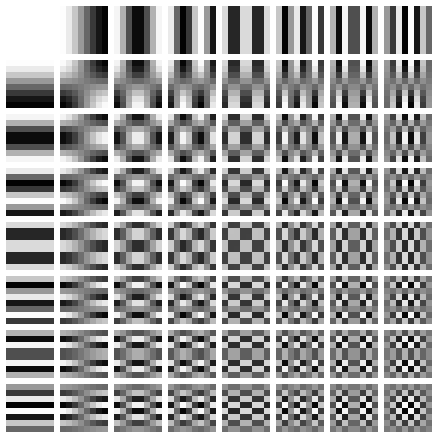
\includegraphics[width=0.5\linewidth]{img/dct-jpeg.png}
            \caption{Częstotliwości DCT dla bloku \(8 \times 8\) obrazu JPEG}\label{fig:dct-basis}
        \end{figure}
    }
\end{itemize}



\nocite{*}
\printbibliography{}

\end{document}
